\documentclass[a4paper]{article}

\usepackage{numprint}
\usepackage{nameref}
\usepackage{float}
\usepackage{url}
\usepackage{graphicx}	% For figure environment
\usepackage{epstopdf}
\usepackage[center]{subfigure}
\usepackage{amssymb}	% For mathematical figures like \mathbb{R}
\usepackage{amsmath}
\usepackage{framed}
\usepackage{tikz}
\usetikzlibrary{mindmap,trees}
\usepackage{pdflscape}
\usepackage[a4paper]{geometry}
\usepackage{subfiles}
\usepackage{listings}
\usepackage{color}

\definecolor{dkgreen}{rgb}{0,0.6,0}
\definecolor{gray}{rgb}{0.5,0.5,0.5}
\usepackage{array}
\usepackage{booktabs}% http://ctan.org/pkg/booktabs
\usepackage{xparse}% http://ctan.org/pkg/xparse
% Rotation: \rot[<angle>][<width>]{<stuff>}
\NewDocumentCommand{\rot}{O{45} O{1em} m}{\makebox[#2][l]{\rotatebox{#1}{#3}}}%
\definecolor{mauve}{rgb}{0.58,0,0.82}

\lstset{frame=tb,
  language=Java,
  aboveskip=3mm,
  belowskip=3mm,
  showstringspaces=false,
  columns=flexible,
  basicstyle={\small\ttfamily},
  numbers=none,
  numberstyle=\tiny\color{gray},
  keywordstyle=\color{blue},
  commentstyle=\color{dkgreen},
  stringstyle=\color{mauve},
  breaklines=true,
  breakatwhitespace=true
  tabsize=3
}


\title{Advanced Systems Lab - Milestone II} 
\author{Matthias Ganz (ganzm@ethz.ch)} 
\date{\today} 


\begin{document}

\maketitle

\pagebreak

\tableofcontents

\pagebreak

\begin{abstract}

This document describes an analytical model of the message queuing system which was build during Milestone I. Analytical studies are presented and compared with the results obtained before.


\end{abstract}

\pagebreak

%% ----------------------------------------------
% Section - The System
%% ----------------------------------------------
\section{The System}

This chapter should briefly show the most important components of the System Under Test (SUT). The curious reader is referred to the document Milestone I. In depth information about the technical details are stated there.


% ------------------------------------------------
% Figure 

\begin{figure}[H]
	\begin{center}
    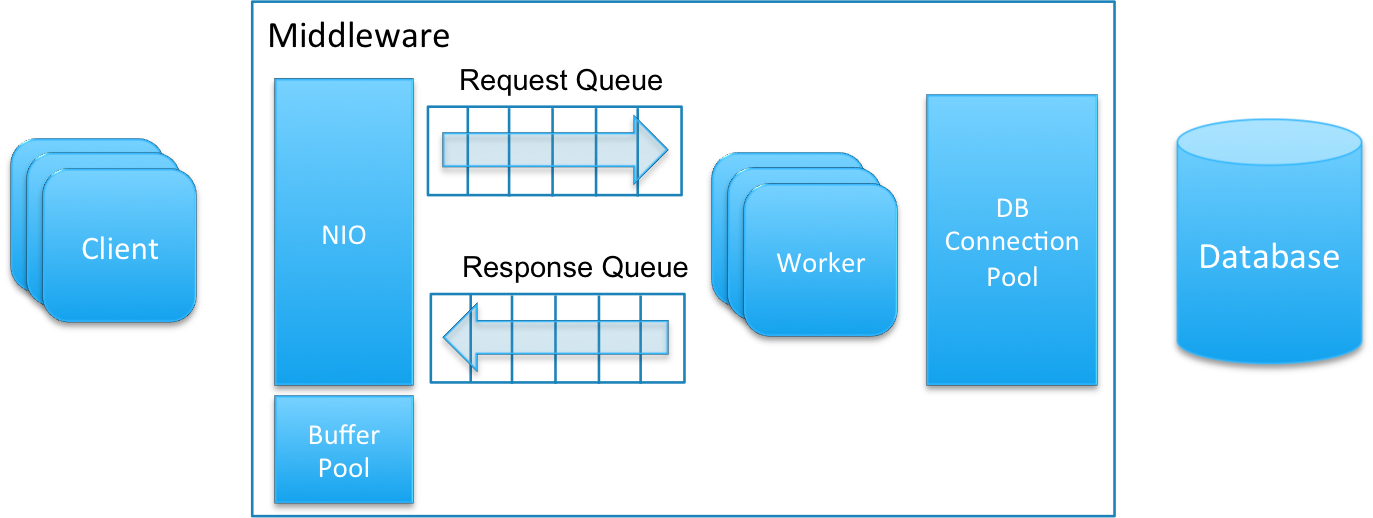
\includegraphics[scale=0.4]{../drawings/broker-threading.png}
  \end{center}
  \caption{System Under Test}
  \label{fig:sut}
\end{figure}

%% ----------------------------------------------

Requests from clients are read and pushed to Request Queue. This Queue is processed by a fixed numer of worker threads which utilize pooled database connections to generate an appropriate response. Theses responses are put back into the response queue which is processed by the networking interface.


%% ----------------------------------------------
% Section System Model
%% ----------------------------------------------
\section{Model of the System}
\label{sec:SystemModel}

\subsection{Modelling a closed system}
Due to the nature of the tests performed during Milestone I the system should be modeled as a closed queuing system. Each experiment was performed with a fixed number of clients. Each client is issuing at max one concurrent request. As long as the system is in its healthy boundaries no messages are discarded by the middleware. Therefore the number of messages in the system never exceed the number of clients.


% ------------------------------------------------
% Figure 

\begin{figure}[H]
	\begin{center}
    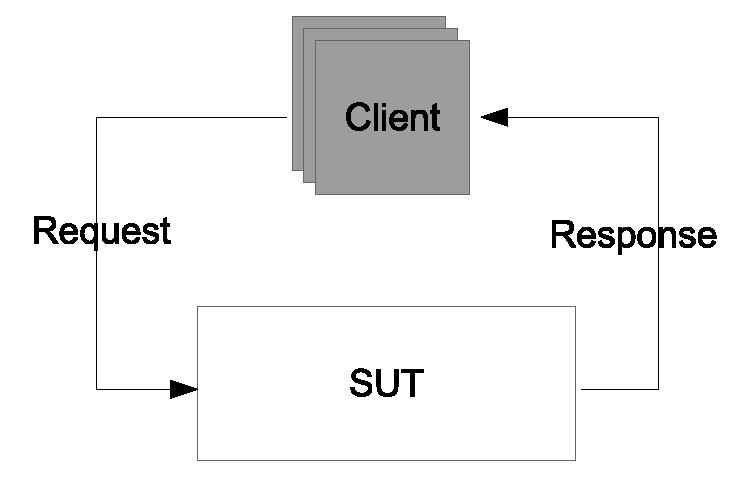
\includegraphics[scale=0.4]{../drawings-ms2/sut.eps}
  \end{center}
  \caption{Closed System}
  \label{fig:closedsystem}
\end{figure}

%% ----------------------------------------------



\subsection{Kendall's Notation}
In this chapter we look at the system as a black box and describe it with \textit{Kendall's Notation}. The 6 characteristic parameters A/S/m/B/K/SD are defined as followed.

\subsubsection{(A) Arrival Process}
\label{subsub:ArrivalProcess}

The interarrivaltime is modeled to be exponentially distributed. This can be shown from figure \ref{fig:interarrivaltime}. Data for this plot where obtained from a shortened 2 hour test with mixed types of clients. From the diagram I assume parameter a) to be \textit{Markovian (M)}.


% ------------------------------------------------
% Figure 

\begin{figure}[H]
	\begin{center}
    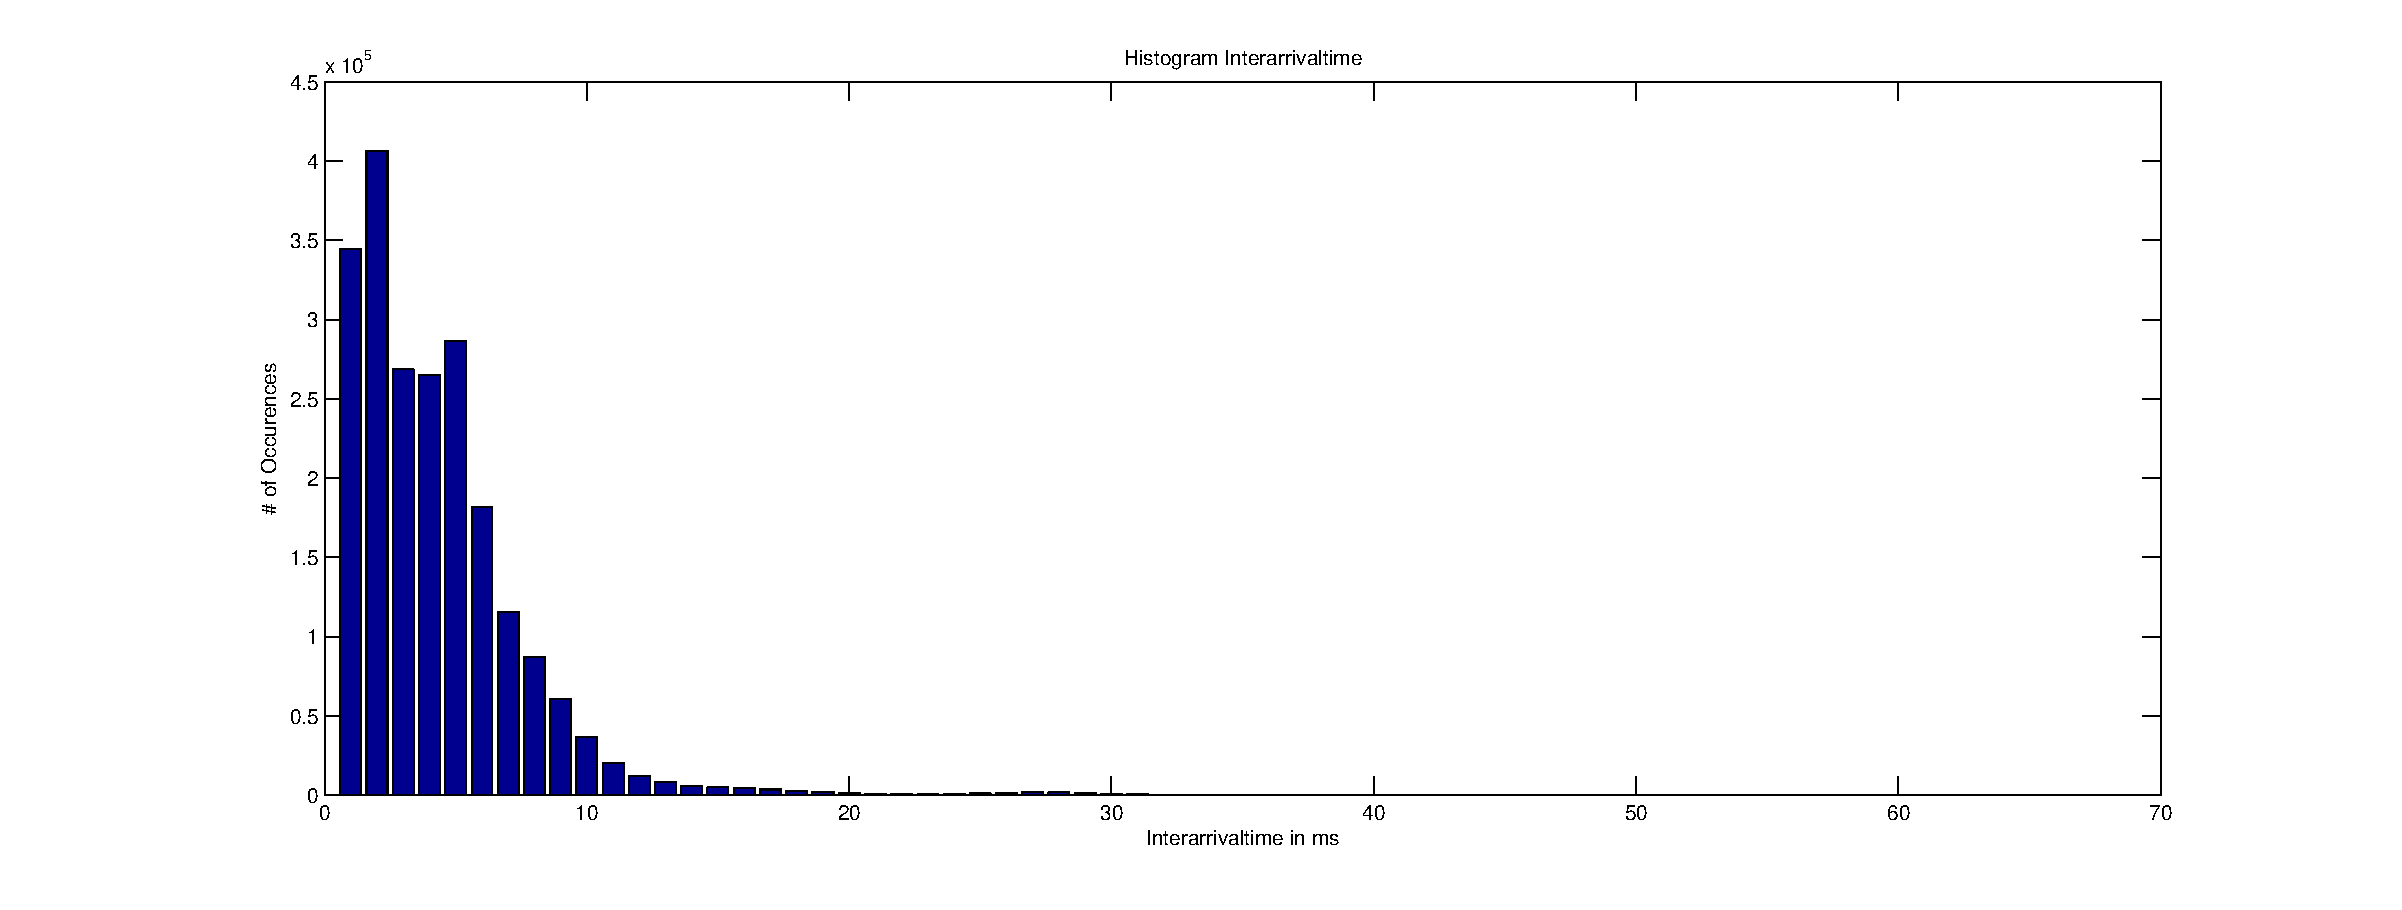
\includegraphics[scale=0.6]{../plots-ms2-mg/interarrivaltime.eps}
  \end{center}
  \caption{Histogram showing Interarrivaltime}
  \label{fig:interarrivaltime}
\end{figure}

%% ----------------------------------------------


\subsubsection{(S) Service Time Distribution }

Again it is assumed that the service time distribution is memoryless exponentially distributed. Data drawn from the same test as in chapter \ref{subsub:ArrivalProcess} show an exponential distribution of service time.

% ------------------------------------------------
% Figure 

\begin{figure}[H]
	\begin{center}
    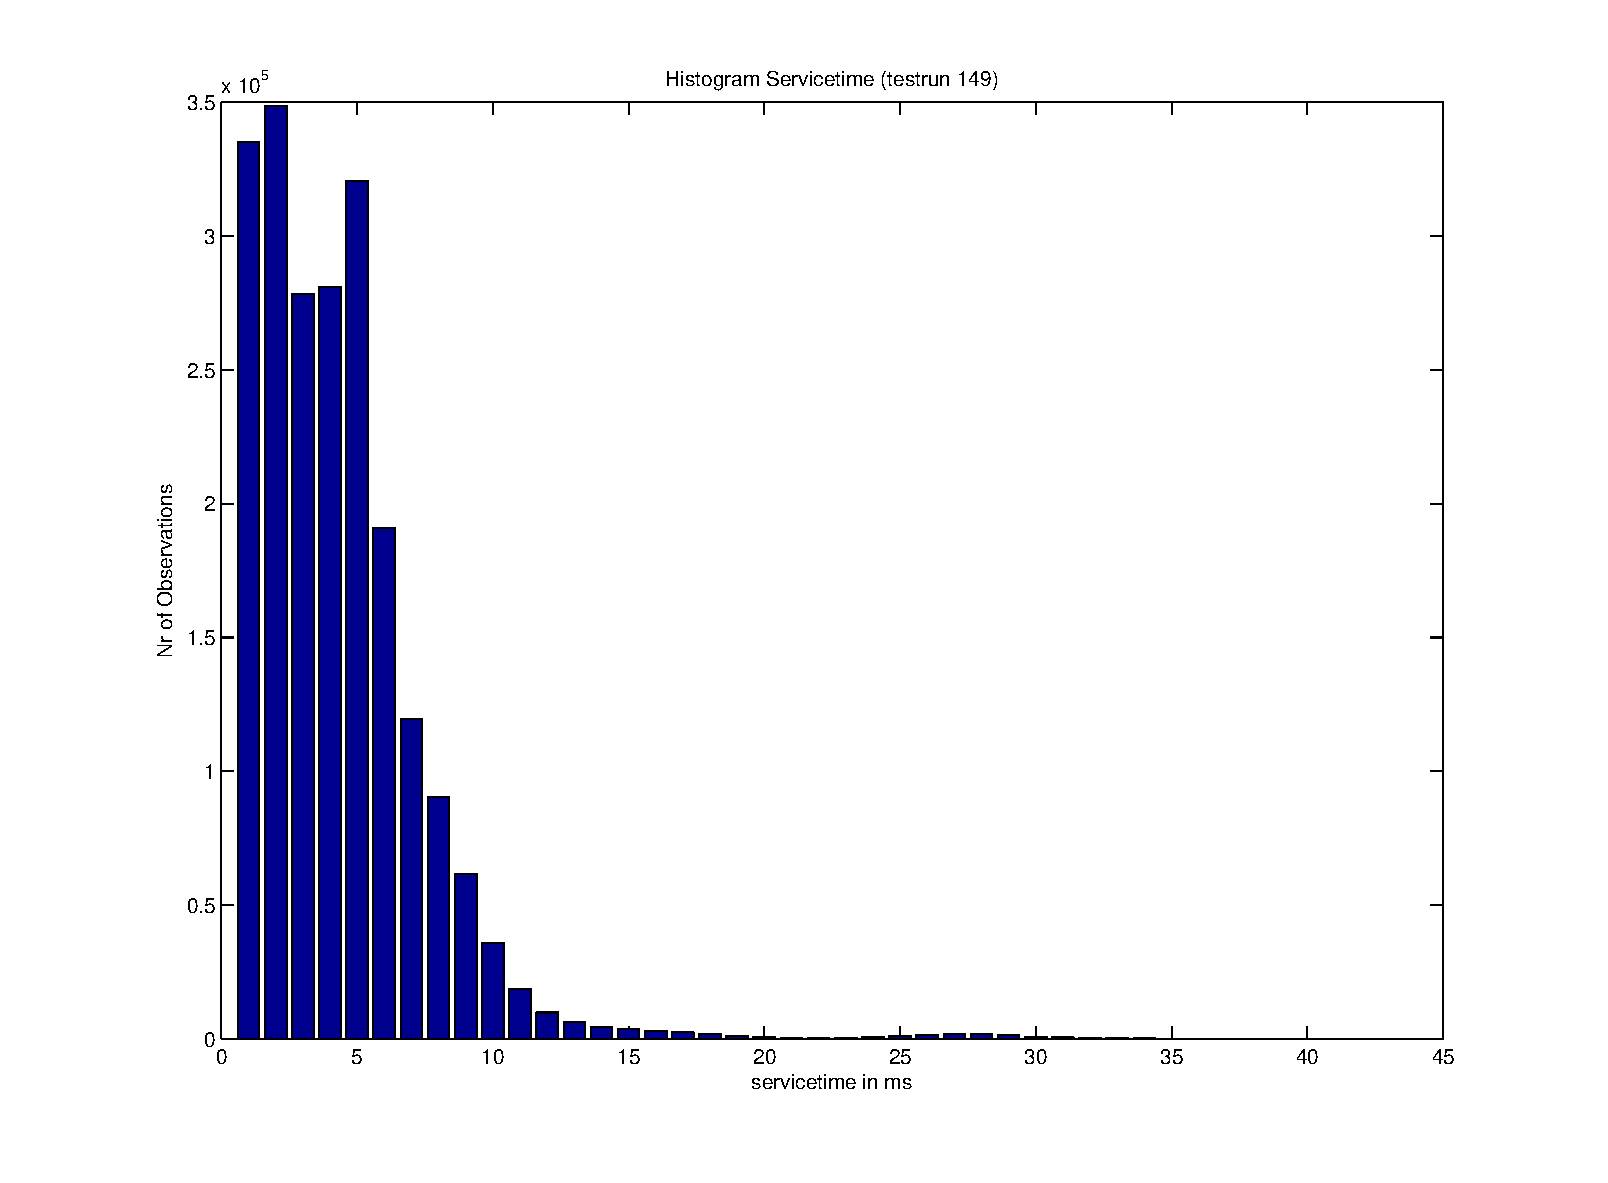
\includegraphics[scale=0.6]{../plots-ms2-mg/servicetime.eps}
  \end{center}
  \caption{Histogram showing Servicetime}
  \label{fig:servicetime}
\end{figure}

%% ----------------------------------------------


\subsubsection{(m) Number of Servers}

This parameter is determine by the number of middleware instances running.

\subsubsection{(B) Buffer - System Capacity }

TODO

\subsubsection{(K) Population Size}

Since we are modelling a closed system the population size can be set to the number of clients participating in the experiment.

\subsubsection{(SD) Service Discipline}
Because the whole messaging system consists of queues  First Come First Server (FCFS) service discipline is assumed for our system model.

\section{Refined System Model}
\label{sec:RefinedSystemModel}

Modelling the system as a black box is not very accurate. To be able to do a more distinct analysis and to identify bottle neck components the black box queue is refined into a queueing network.

Figure \ref{fig:systemmodel-singlebroker} shows the model of the system with only one middleware instance. It is modelled having four different service centers which are described in the following subsection.

% ------------------------------------------------
% Figure 

\begin{figure}[H]
	\begin{center}
    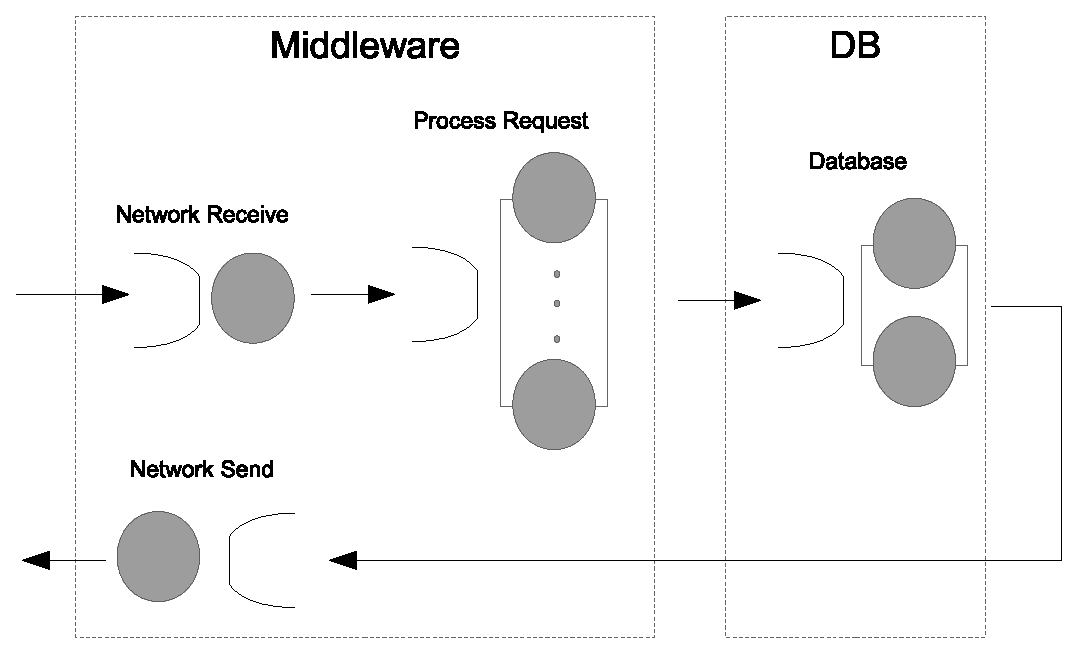
\includegraphics[scale=0.6]{../drawings-ms2/systemmodel-singlebroker.eps}
  \end{center}
  \caption{System Model with one Middleware}
  \label{fig:systemmodel-singlebroker}
\end{figure}

%% ----------------------------------------------

\subsection{Service Centers}

\subsubsection{Client}
The clients are modelled as Delay Centers. The time a client is sleeping between two requests is the think time $Z$.

\subsubsection{Network Receive}
\label{subsub:ServiceCenterNetworkReceive}

This service center represents the networking part where the middleware gets a request and buffers it until completely received. For this queue also the time used sending the request over the network is taken into account. The number of service nodes is 1 because receiving and buffering is done single threaded by the nio networking interface.\\

\begin{tabular}{|l|l|}
\hline 
Type & fixed capacity \\ 
\hline 
Queue Size & unbound\\ 
\hline 
Service Node Count & 1 \\ 
\hline 
\end{tabular} 

\subsubsection{Process Request}
This service center represents the request queue and the worker threads attached to it. The queue is represented by an actual queue and workers implemented in java. The queue size is fixed and corresponds with the size of the java queue (which is configurable and by default set to 100) \\

\begin{tabular}{|l|l|}
\hline 
Type & load dependent \\ 
\hline 
Queue Size & Corresponds to Request Queue size (default 100)\\ 
\hline 
Service Node Count & Corresponds to \# of worker thread \\ 
\hline 
\end{tabular} 

\subsubsection{Database}
This node represents the database. For the experiment an Amazon medium instance with two ECU's (EC2 Compute Units\footnote{Assumed to something equivalent to a CPU. Actually Amazon does not further explain the term ECU.}). The queue size is modelled to be infinite. The number of service nodes is set to 2.\\


\begin{tabular}{|l|l|}
\hline 
Type & fixed-capacity service center \\ 
\hline 
Queue Size & unbound \\ 
\hline 
Service Node Count & 2 \\ 
\hline 
\end{tabular} 


\subsubsection{Network Send}
This service center represents the networking part where the middleware sends back a response. Responses to transmit are buffered in a java response queue. So the queue size corresponds to the size of the java queue. As in section  \ref{subsub:ServiceCenterNetworkReceive} the service node count is one. \\

\begin{tabular}{|l|l|}
\hline 
Type & load dependent \\ 
\hline 
Queue Size & Corresponds to Response Queue size (default 100)\\ 
\hline 
Service Node Count & 1 \\ 
\hline 
\end{tabular} 

\subsection{Modelling Multiple Middlewares}

The model shown in section \ref{sec:SystemModel} takes only one middleware into account. Since clients are evenly distributed among multiple stateless middlewares and the visit ratio $V_i$ of the $i$-th queue for $n$ instances is $1 \over n$ we can simplify the model by merging all of them together. This means that for each broker added the queue size and service node count is increased accordingly. This assumption is backed by the Forced Flow law. In a closed system no request leaves the system.

\paragraph{For example} if there are 8 middleware the queue size of the \textit{Network Receive} component is still unbound but the service node count is 8 instead of 1 (it becomes a load dependent service center).

%% ----------------------------------------------
% Section Single Queues
%% ----------------------------------------------
\section{Analysing the Queues}

To further analyse the queues defined in section \ref{sec:RefinedSystemModel} the experiment described in section \ref{sec:experiment} with a client count of 120 was taken. All measurement values used here are taken from there.

\subsection{Network Receive - M/M/8}
Since we scale the number of middlewares to 8 this queue becomes a M/M/8 queue. The queue size is still infinite.


From the experiment the following values were measured:

\begin{tabular}{|c|c|c|}
\hline 
$\lambda$ & mean arrival rate & TODO \\ 
\hline 
$\mu$ & mean service rate & TODO \\ 
\hline 
$m$ & number of service nodes & 8 \\ 
\hline 
\end{tabular} 

\subsubsection{Traffic intensity $\rho$}

$$ \rho = \lambda / (m \mu) = TODO$$

Since $\rho$ is below 1 this system is stable.


See \cite[Box 31.2]{Raj}


\subsection{Network Receive - M/M/8}

\subsection{Process Request - M/M/8* / 100*8}

\subsection{Network Receive - M/M/8}

\subsection{Network Receive - M/M/8}

\begin{tabular}{|l|l|}
\hline 
$\lambda_{rx}$ & arrival rate in requests per minute \\
\hline 
$\mu_{rx}$ & service rate of a single service node in requests per minute \\
\hline 
$m_{rx}$ & number of service nodes \\
\hline 
\end{tabular}

Traffic intensity $\rho = {\lambda} / {(m \mu)}$ should be less than 1.

%% ----------------------------------------------
% Section Bottleneck Analysis
%% ----------------------------------------------
\section{Bottleneck Analysis}

A bottleneck analysis was performed to determine which component limits the total capacity of the system. Table \ref{tabular:BottleneckParams} shows the values required for this Analysis.

Row $S$ and $X$ are measurement values obtained from Milestone I. By applying \textit{Utilisation Law} (eq. \ref{eq:UtilisationLaw}) row $U$ can be calculated.   

\begin{equation}
\label{eq:UtilisationLaw}
U = X S
\end{equation}


The last row $D$ is obtained by combining \textit{Utilisation Law} and \textit{Forced Flow Law} (eq. \ref{eq:Demand}). 

\begin{equation}
\label{eq:Demand}
U = X_{total} D
\end{equation}


\begin{figure}[H]
\label{tabular:BottleneckParams}
\begin{center}
\begin{tabular}{|l|l|l|l|l|l|}
\hline 
 & \textbf{Network Receive} & \textbf{Process Request} & \textbf{Database} & \textbf{Network Send}\\ 
\hline
\textbf{$S$ Mean Service Time [ms]} & • & • & • & • \\
\hline 
\textbf{$X$ Throughput [req/min]} & • & • & • & • \\
\hline
\textbf{$U$ Utilisation} & • & • & • & • \\
\hline
\textbf{$D$ Demand} & • & • & • & • \\
\hline
\end{tabular} 
\caption{Bottleneck Analysis Input Parameters}
\end{center}
\end{figure}


- Mean Service Time per Device $S_i$\\
- Throughput per Device $X_i$


%% ----------------------------------------------
% Section MVA
%% ----------------------------------------------
\section{Mean-Value Analysis}

A Mean-Value Analysis was performed for the system. According to \cite[Box 31.2]{Raj} the following input parameters of the system are needed.

\begin{tabular}{|c|c|}
\hline 
$Z$ & Thinktime \\ 
\hline 
$S_i$ & Service timer per Visit \\ 
\hline 
$V_i$ & Number of Visits \\ 
\hline 
M & Number of Devices \\ 
\hline 
N & Number of User \\ 
\hline 
$\mu_i(j)$ & • \\ 
\hline 
• & • \\ 
\hline 
\end{tabular} 



\subsection{Measured Values}

\begin{tabular}{|l|l|}
\hline 
$N$ & Number of clients in the system \\ 
\hline 
$X$ & Total throughput in requests per second \\ 
\hline 
\end{tabular} 

\begin{tabular}{|c|c|c|c|c|}
\hline 
$N$ & $X$ & • & • & • \\ 
\hline 
30 & • & • & • & • \\ 
\hline 
60 & • & • & • & • \\ 
\hline 
90 & • & • & • & • \\ 
\hline 
120 & • & • & • & • \\ 
\hline 
120 & • & • & • & • \\ 
\hline 
\end{tabular} 

\subsection{Service Times}

\begin{tabular}{|c|c|c|c|c|}
\hline 
  & Network Receive & Process Request & Database & Network Send \\ 
\hline 
Mean service time $S$ & • & • & • & • \\ 
\hline 
Visit Ratio $V$ & • & • & • & • \\ 

\hline 
\end{tabular} 


- balanced job bounds

%% ----------------------------------------------
% Section Experiments
%% ----------------------------------------------
\section{Experiment}
\label{sec:experiment}
For this milestone it was decided to repeat the experiment where the load is gradually increased until the system trashes. The previous one performed for milestone 1 was flawed because the number of clients were dynamically increased without stopping the measurements. Warmup time of the freshly connected clients were not considered properly.

\subsection{Experiment Setup}


\begin{figure}[H]
\label{tabular:experimentsetup}
\begin{center}
\begin{tabular}{|l|l|}
\hline 
\textbf{Parameter} & \textbf{Value} \\ 
\hline 
Broker & 8 distributed over 4 Amazon EC2 medium  instances (2 VCU per instance)\\ 
\hline 
\# of Worker Thread & 20 per middleware \\
\hline 
\# of DB Connections & 15 per middleware \\
\hline 
Client Type & OneWayClient \\ 
\hline 
Client Think Time & 10ms \\ 
\hline 
\# of Clients & 30 - 450 \\ 
\hline 
Request Timeout & 1 s
\hline 
Experiment Duration & 7min \\ 
\hline 
\end{tabular} 
%\caption{Experiment Parameters}
\end{center}
\end{figure}


\subsection{Hypothesis}

By increasing the load on the system both response time and throughput should increase to
a certain degree. By increasing the load more the system should become unstable and start
trashing.

\subsection{Result}


\begin{tabular}{|l|l|}
\hline 
TestRunId & \# of Clients \\ 
\hline 
191 & 30 \\ 
\hline 
\end{tabular} 

\subsection{Sanity Check}

The measured data can be check if they are plausible using the \textit{Interactive Response Time Law}.

\begin{equation}
\label{eq:InteractiveResponseTimeLaw}
X = {{N} \over {R + Z}}
\end{equation}


Where $X$ is the throughput, $N$ the number of clients, $R$ the response time and $Z$ the think 	time. Table \ref{tabular:experimentsanitycheck} shows the table containing the measured values. Column $Z$ with the think time was calculated using formula \ref{eq:InteractiveResponseTimeLaw}. 

\begin{figure}[H]
\label{tabular:experimentsanitycheck}
\begin{center}
\begin{tabular}{|l|l|l|l|}
\hline 
$N$ & $X$ [req/min] & $R$ [ms] & $Z$ [ms]\\
\hline 
30&	49970&	20&	16\\
60&	85833&	32&	10\\
90&	94047&	48&	9\\
120&	99332&	60&	12\\
150&	101191&	72&	17\\
180&	99415&	92&	17\\
210&	98858&	109&	18\\
\hline 
\end{tabular} 
\caption{Calculated Think Time}
\end{center}
\end{figure}





\subsection{Interpretation}

TODO - describe graphs\\

The calculated think time has the expected magnitude and does not vary too much (around 15ms). The measured data seem to be plausible.

%% ----------------------------------------------
% Section MEMOS
%% ----------------------------------------------

\pagebreak

\section{Memos}

open or closed system
- do we have an open or a closed system? It's closed!

- use bullshit word "service center"

- build alanytical queuing model of the whole system
  - parameters
- build alanytical queuing model for each part of the system
  - parameters
- explain where data matches the model and where not

- interactive response time law, not applicable because of client implementation

analytical model, 


- network of queues
  - not too fine, abstract away threads
  
  
- explain why the model matches reality (or not)


- siehe buch seite 1078 fuer Anregungen was man so machen müsste

Sample book ref \cite[Page 556]{Raj}


\bibliographystyle{plain}
\bibliography{literature}


\end{document}

